\documentclass[conference]{IEEEtran}
\IEEEoverridecommandlockouts
% The preceding line is only needed to identify funding in the first footnote. If that is unneeded, please comment it out.
\usepackage{cite}
\usepackage[letterpaper, left=0.68in, right=0.68in, bottom=1.049in, top=0.75in]{geometry}
\usepackage{amsmath,amssymb,amsfonts}
\usepackage{algorithmic}
\usepackage{graphicx}
\usepackage{cleveref}
\usepackage{textcomp}
\usepackage{xcolor}
\usepackage{siunitx}
\begin{document}

\title{Experimental validation of L3 VPN Network Model for improving VPN service design and provisioning}

\author{\IEEEauthorblockN{Samier Barguil}
\IEEEauthorblockA{\textit{Universidad Autonoma de Madrid}\\
Madrid, Spain\\
samier.barguil@estudiante.uam.es}\\
\and
\IEEEauthorblockN{Oscar Gonzalez de Dios \\
and Victor Lopez Alvarez}
\IEEEauthorblockA{\textit{Telefonica I+D}\\
Madrid, Spain}\\
\and
\IEEEauthorblockN{Roque Gagliano and Ignacio Carretero}
\IEEEauthorblockA{\textit{Cisco Systems}\\
Pully, Switzerland and Madrid, Spain}\\
\and
\IEEEauthorblockN{Ricard Vilalta}
\IEEEauthorblockA{\textit{Centre Tecnologic de Telecomunicacions de Catalunya (CTTC/CERCA)} \\
Casteldefels, Spain}\\
}
\maketitle
\begin{abstract}
Current approaches to automate the design and configuration of transport services face several challenges. Firstly, there is a lack of open interfaces between the Operational Support Systems (OSS) and the network layer. The commercially available interfaces to Network Management Systems (NMSs) or directly to the devices are typically proprietary and with limited programmability. Secondly, for the case of IP/MPLS networks, the definition of how a service is built is particular to each operator.

To solve this situation, this work presents an approach based on a hybrid SDN in which the definition of a VPN service is made with a modeling language and is not limited to a particular operator design nor a particular set of vendor devices. The IP/MPLS network topology and the VPN services are programmable via standard APIs with RESTCONF/YANG from an SDN Controller. This facilitates the operator on the one hand designing a new VPN service and its full automation.  This work demonstrates, for the first time, that such automation is possible with proposed draft standards from IETF and validates its implementation, comparing the time consumed in the controller to process to different workflows from the same model.
\end{abstract}

\begin{IEEEkeywords}
L3VPN, IP Networks, SDN, Service Provisioning
\end{IEEEkeywords}

\section{INTRODUCTION}
Network operators are in continuous evolution to satisfy the changing and variable service demands of the end-users. Such evolution affects not only to the service offering but also to the network supporting the delivery of such services. A crucial part of this network is the transport infrastructure. Transport networks are responsible for forwarding aggregated traffic demands from end-users consuming different services across cities, regions, or continents. Transport network architecture was conceived for static scenarios, where were the traffic patterns usually follow the preconceived flow. This assumption allows configuring the network as a slow process since there was no need for the operator to reconfigure the deployed resources dynamically.

Software-Defined Networking (SDN) originally \cite{brief2014openflow,gude2008nox,tavakoli2009applying} came with the concept of the decoupling of control and forwarding planes in the network elements. A centralized controller with the complete network view does the control plane functions. It runs intelligent algorithms and applications (either as part of the controller or on top of it) and instructs the nodes accordingly. This original view, when ported to real carrier networks \cite{bemby2015vino}, has been evolved slightly towards an architecture where the centralized control assists the network elements on the forwarding tasks. This hybrid SDN approach provides a single and unified control environment for network operations and at the same time, optimizes the usage of network assets. The network elements yet retain control capabilities (in some cases, alleviating some signaling tasks), but leveraging on the centralized controller for end-to-end and cross-layer actions through programmable interfaces. 

The use of the SDN principles is aimed to simplify the network operation and to allow a fast reaction and adaptability to network changes motivated by traffic variability or simply because of service configuration. Besides network element control functions, SDN is also considered as an entity to provide support for management functions, such as a collection of real-time information that could permit the automatic configuration creation and activation in network elements, as triggered by the Operational Support Systems (OSS). Day to day network operation for a service provider involves a set of complex and technologically specific tasks. Some of these include periodic operations as capacity planning, traffic forecast analysis, network convergence optimization, new devices installation, or routine tasks like troubleshooting, patching, support in maintenance windows, or service provisioning. Commonly, the first set of tasks requires a high specialization and in-depth technological knowledge. However, the second set is mainly repetitive. 

Since years ago, the usage of scripts to automate network tasks has become common. The usage of those scripts combined with some automation frameworks such as Ansible \cite{libes1995exploring} or libraries like Expect \cite{hochstein2017ansible} or Paramiko \cite{zadka2019paramiko} are the highest level of automation found in service providers. Lately, similar works has been done using more modern tools such as NETCONF/RESTCONF \cite{enns2011network,bierman2017RESTCONF,vilalta2018experimental} interfaces and YANG \cite{bjorklund2016yang} abstract models. Some of the works available are focus, on solution the  Layer-2 services (L2VPNs) provision \cite{ventre2017sdn,noghani2017automating,wuframework} and/or Layer-3 Services (L3VPNs), including some new features such as the 5G deployment \cite{rokui2020standards}.

%%In paralel some DevOps teams have been created to reduce the volume of manual task. However, some studies have revealed that even if the tools used between Service Providers are the same and the set of services configured are the same Virtual Leased Lines (VLL), Layer-2 services (L2VPNs) and Layer-3 Services (L3VPNs), there is not a common way to do it. In that sense, due to the high level of customization, automation has implementations not easy to replicate between companies or even teams in the same company. 

%%To solve this problem, several YANG models have been released to support the service provisioning based on NETCONF/RESTCONF \cite{enns2011network,bierman2017RESTCONF} interfaces and YANG \cite{bjorklund2016yang} abstract models. 

In this paper, we present the intent-based configuration of the MPLS L3 VPN services in a carrier grade ecosystem. A commercial SDN domain controller using RESTCONF NBI (Northbound Interface) is tested. The controller implements a YANG network model named L3NM (A Layer 3 VPN Network YANG Model) used to abstract the complexity of the network configuration.  As the main result of this work, the time consumed by two ways to use the same YANG data model to request and delete the service at controller and network level were compared.

This paper has the following structure: \Cref{sect:arqu} explains the functional architecture for an IP SDN solution. \Cref{sect:l3vpn} explains the Network Service Models used for the L3VPN definition. \Cref{sect:exp} explains the experimental validation and the results obtained. Finally, \cref{sect:conclu} concludes this paper. 

\section{ARCHITECTURAL PROPOSAL}
\label{sect:arqu}

IP networks usually follow a hierarchical model, mixing equipment from different vendors. The IP routers are interoperable at data and control plane level (e.g., routing protocols such as IS-IS, OSPF, or BGP). Due to scalability reasons, the IP networks have in IP subdomains to confine the routing and control protocols on their particular domains.

\begin{figure}
	\centering
		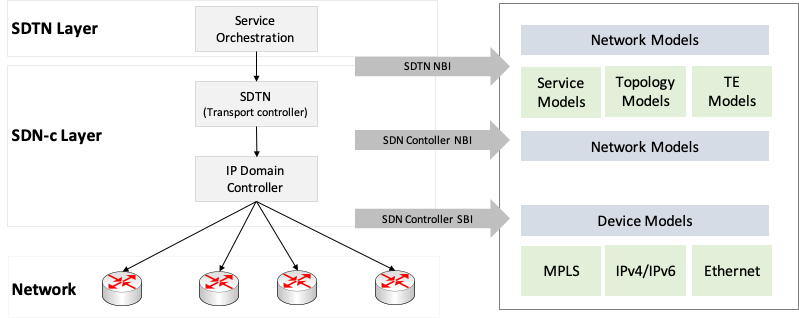
\includegraphics[width=\linewidth]{fig1_architecture.png}
	\caption{IP SDN Domain Controller deployment}
	\label{FIG:1}
\end{figure}


\Cref{FIG:1} shows the role of IP SDN Controller (IPSDNc) under the iFusion network architecture defined in \cite{contreras2019ifusion} by Telefonica. This architecture solution focuses on a single, multi-vendor controller responsible for configuring the IP network elements. The Northbound Interface (NBI) of the controller is based on standard models defined in YANG. To access it, the protocol supported is RESTCONF with JSON encoding.

The NBI allows the programmatic configuration of all elements participating in a service. Thus, the IPSDNc must handle the service creation requests delivered by the service orchestration layer and translate it to device-specific configuration. For this task, the target Southbound Interface (SBI) of the IPSDNc is to make a vendor-agnostic device configuration using the NETCONF protocol and a common data model. The set of device configuration data models for the IP segment is still under development, but a lot of YANG definitions have been made in Openconfig or IETF until now. 

\section{LAYER 3 VPN PROVISIONING}
\label{sect:l3vpn}

The Layer 3 Virtual Private Network (VPN) service defined in RFC 4364 \cite{rosen2006rfc} provides a multipoint, routed service to the customer over an IP/MPLS core. The L3VPNs are widely used to deploy 4G/5G, fixed, and enterprise services, principally because, not only many traffic discrimination policies can be applied to transport but also because of several stitching methodologies can be applied to combine access and transport services. 

\begin{figure}
	\centering
		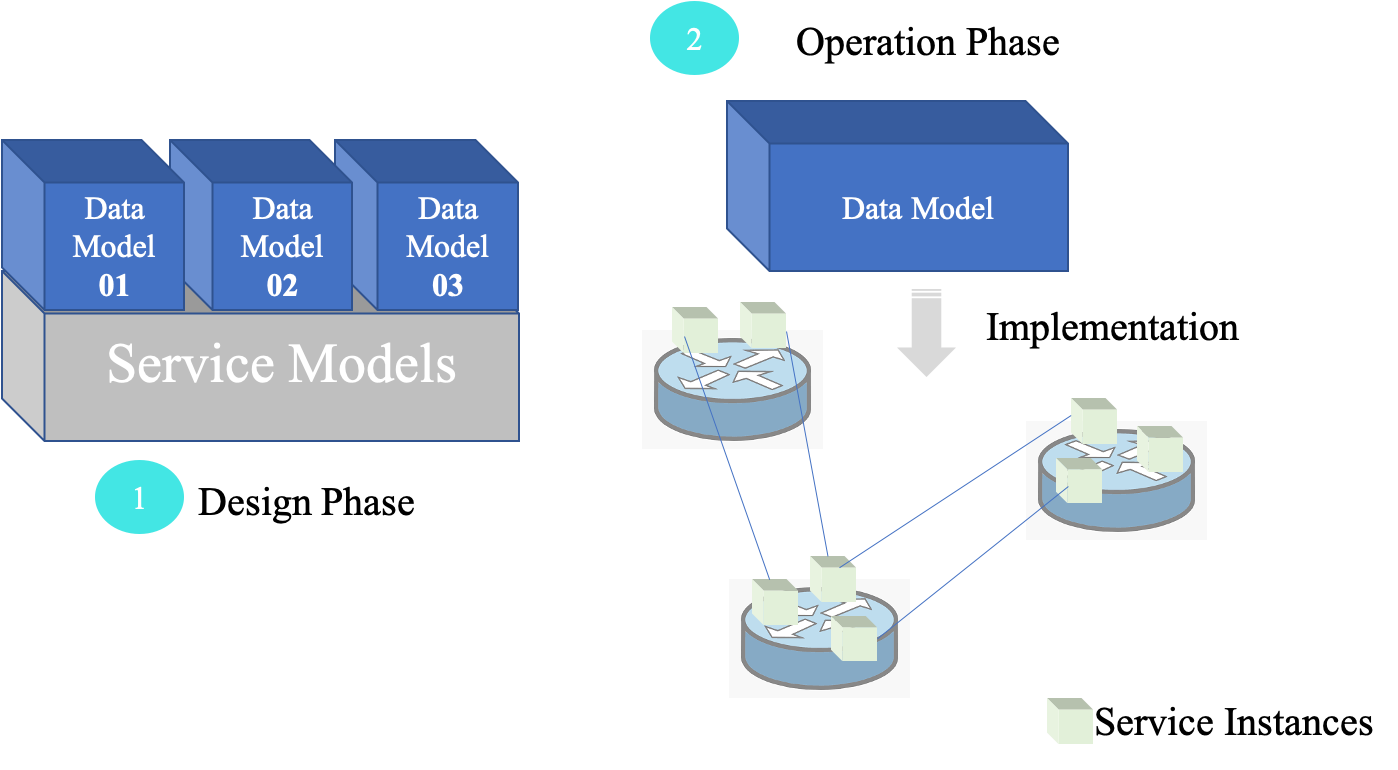
\includegraphics[scale=0.3]{figure2png.png}
	\caption{Design Phase and implementation phases of a MPLS VPN Service}
	\label{FIG:2}
\end{figure}

To improve the L3VPN lifecycle management in the service provider network, as depicted in \cref{FIG:2}. Two phases need to be analyzed:
\begin{itemize}
    \item Design phase: Some service models have been defined and standardized until now. These works include generic purpose modeling languages like TOSCA or YANG.
    \item Operation phase: Instantiate the Service requests on the devices and operate them in the live network. It implies the ability to reuse the same service models against devices from different vendors.
\end{itemize}

These two phases can be executed in different timeframes. However, the set of requirements and parameters defined in the design limits the degree of automation provided during the implementation phase. 

\subsection{Design Phase: Layer 3 VPN Network API}

L3NM \cite{Aguado:2019aa} is a YANG data model to manage and control the VPN Service configuration based on the service provider requirements:
\begin{itemize}
    \item Create a VPN Service
    \item Provision VRF on the PE
    \item  Attach the interface to the PE
\end{itemize}


The L3NM model is Network Centric and it is focused on the service provider internal network parameters. By definition, the data model can be used to facilitate communication between the service orchestrator and the Network. The L3NM model does not keep any of the commercial customer parameters which belong to the OSS/BSS layer.

\subsection{Operation phase: SBI Models Support}

To instantiate the services on the devices notably YANG data models are available from standard bodies such as IETF, Broadband Forum, 3GPP, MEF and others. Additionally, a number of interest groups have been formed in recent years to create common data models for a specific group of interest. This is the case of OpenConfig which started by addressing the needs of Cloud Service Providers but is now expanding to network service providers and beyond. 

As in any standard, data models will not address all the capabilities of any given devices. Therefore, device vendors are implementing their own (many times called native) data models that do cover all the capabilities for a given device type and operating system version.

The typical way these overlaps of different YANG models are implementing is by a native implementation of NETCONF with direct or indirect (for example via the CLI API) access to the configuration database. Consequently, there are several nuances that operators need to be aware when planning which southbound data models to select:
\begin{itemize}
    \item Typically, only the native data models provide full access to all the device capabilities. This is especially true for some innovative or recent features.
    \item There will be overlaps where a single configuration object (let’s say interface configuration) can be accessible via different modules. 
    \item As the semantic of the different modules are not guaranteed to play well together, a clean cut between modules for a “mix scenario” is not given.
\end{itemize}

For those use cases where we have defined a target southbound data model, we also need to consider the lifecycle management of these modules, in special as:
\begin{itemize}

\item Device vendors will deviate between themselves on what and how they implement standard data models. These deviations are supported by the YANG specifications but in essences means that for a controller, two southbound standard data models would not be equal. 

\item Device vendors will deviate on how they implement the different data models (even native) across their platforms and operating systems versions. Different platforms and operating system versions have different hardware and software capabilities, and therefore cannot expose the same APIs.

\item YANG data modules evolve into new releases, these new releases may or may not follow the RFC6020 and RFC7950 rules for module upgrade. This means that the same namespace may have different meanings depending to which device you are talking to, which violates one of the main principles for YANG (RFC 7950 section 5.3).
\end{itemize}

The NETCONF/YANG standards do not mandate any specific “workflow”, i.e. if the target configuration should be executed as “all at once” or in a specific sequence. Moreover, dependencies between nodes in a YANG models are not annotated via any standard capability. This means that two standard compliant vendors may require different number of total commits for the same target configuration.

We can now summarize then what should we require from a NETCONF/YANG southbound implementation in a network controller (besides supporting the mandatory standard documents) to make it functional in current real deployment scenarios:
\begin{enumerate}
    \item The controller should be able to support southbound devices that provide their own mix of standard and non-standard device data models, where the operator should be free to choose what combination it desires for every device group.
    \item The controller should support multiple copies for the same namespace to allow different implementations across device types and vendors.
    \item The controller should support by default the “all at once” single step. Conversely, the controller should support devices that require multiple commits via a different behavior.
\end{enumerate}

\begin{figure}
	\centering
		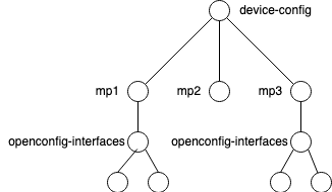
\includegraphics[scale=0.9]{figure3.png}
	\caption{Schema mount in RFC8528 used to map two implementations of openconfig-interfaces as SBI}
	\label{FIG:3}
\end{figure}

One of the main technologies that may help vendors to address these concerns is the use of the YANG Schema-Mount standard (RFC8528). Thanks to this technology, different versions of the same namespace could be added to different nodes in the controller configuration and state trees. This means that if we create a list of implementation, we could “mount” as many variants as desired. The idea of using the YANG Schema-Mount was already introduced at the Broadband Forum (BBF) TR-413 specification for the Broadband Access Abstraction (BAA) layer. In that document, the BBF also suggest the use of the same technology to solve the implementation of multiple protocols southbound (CLI, SNMP, REST) and mapping them to a common YANG representation depicted in \cref{FIG:3}.

\section{EXPERIMENTAL VALIDATION}
\label{sect:exp}
The network set-up and the test done are explained in this section.

\subsection{Network Set-up}
For our experiments, we have chosen the OpenConfig data models for Cisco IOS-XR and the Cisco Network Services Orchestrator (NSO) as the IP Controller. The Cisco NSO controller implements the YANG Schema-Mount standard (RFC8528) southbound and the L3NM as the service model in the NBI.

\subsection{L3VPN Provisioning Workflow}

The L3NM uses the YANG Modeling Language to describe an MPLS L3VPN service. The model defines two main containers, one for sites and one for the VPN-services. Each of these containers includes a list to create a set of sites and services, respectively. Each item (site or service) is uniquely identified in the list by their id.

The segmentation between site and services in the model design allows the re-utilization of sites between several services and allows several degrees of flexibility to request services based on intents.  For example, an intent can be used to provision the sites and make the PE-locations available for the controller, and a second intent to create the VPN service itself.

\subsection{Experimentations}
To evaluate the YANG model defined for the L3VPN and how its design can impact the service instantiation, the following tests were done:
\begin{enumerate}
    \item Define the minimum set of intents to request the service: Based on the YANG model structure, the minimum number of intents required to complete the VPN onboarding process is three (3).
    \item Compare the minimum set of Intents against the number of calls suggested by the model creators: The model specification suggest five (5) intents as the optimal number of requests. 
    \item Create a hundred (100) services/tests using both provisioning methodologies and capture the time consumed by the controller to process each service request, measured as:
    \begin{equation}
         \si{\textrm{Net time}= \textrm{Creation} + \textrm{Deletion}\qquad \second}
    \end{equation}
\end{enumerate}

\begin{figure}
	\centering
		\includegraphics[width=\linewidth]{figure41.png}
	\caption{Intents and numbers of parameters used in each test}
	\label{FIG:4}
\end{figure}

Based on this, two workflows to request the VPN service to the network controller were defined. The workflows differ on N the number of calls done to create the service but globally the total number of parameters is identical, as detailed in \cref{FIG:4}.

Each workflow follows the next steps:  ALl the creation intents are sent to the IPSDNc using RESTCONF/YANG. IPSDNc computes the call and, if the request is valid, the controller returns the creation confirmation code. The network controller does the service deployment on the network only when the intent related to the VPN-Network-Access is received. The other intents create resources at the controller level only.

\begin{figure}
	\centering
		\includegraphics[width=\linewidth]{figure51.png}
	\caption{Performance results obtained during the testing}
	\label{FIG:5}
\end{figure}

\begin{figure}
	\centering
		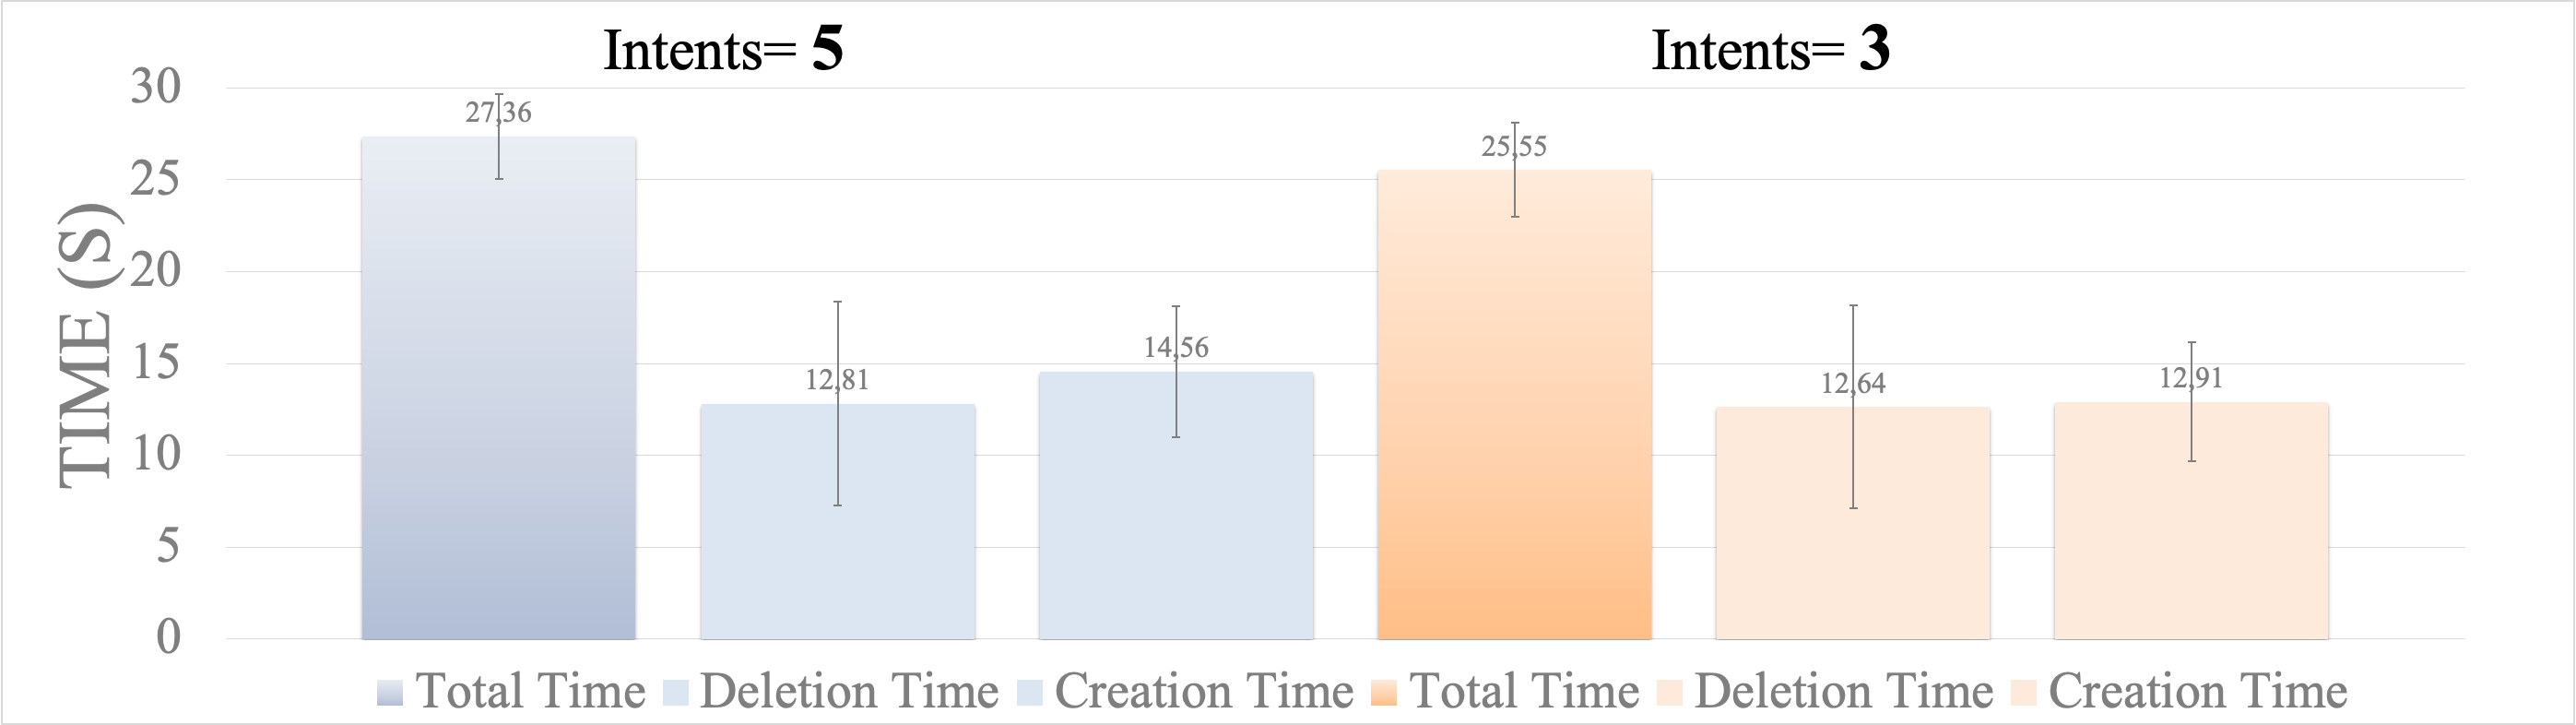
\includegraphics[width=\linewidth]{figure62.png}
	\caption{Performance results obtained during the testing}
	\label{FIG:6}
\end{figure}

\section{RESULTS}
\label{sect:resul}

The total time consumed by the IPSDN controller to create and delete a VPN service form the network was measured. The mean $u$ values and the standard deviation $d$ is computed in the for the 100 experiments as depicted in \cref{FIG:5}. The main difference was found during the creation process. During creation, each additional call introduces a delay of $0,82$ seconds per additional call. This number seems low, however a change in the model structure, for example, avoid the cross-references between the containers of sites and VPN services, can allow a single call creation process. This potentially will reduce the creation time, a bit more. This kind of behavior can be treated as a design rule to make the model implementation efficient. 

\section{CONCLUSIONS}
\label{sect:conclu}

Telecommunication providers are forced to continuously evolve their networks to provide a better service for their customers. Thus, Network automation initiatives are highly necessary.  The implementation of these initiatives requires their adaptability and support of brownfield scenarios in operating networks. This support must include not only the configuration of the devices and all the possible services provisioned in the day-to-day operations across the service provider networks. 

Firstly, this article provides an overview of the latest state-of-the-art standardization efforts of the L3 VPN life cycle management. Secondly, the work implements for the very first time the L3NM. Two workflows were used to request the service using the same network model. The time consumed using each workflow to implement the service on the device were measured and compared. The work demonstrates that YANG design rules can directly affect the time consumed to create services and explains how device models implementations can limit the deployment of common interfaces

\section*{Acknowledgment}
This work was supported partially by the European Commission H2020-ICT-2016-2 METRO-HAUL project (G. A. 761727) and Spanish AURORAS (RTI2018-099178).

\bibliographystyle{ieeetr}
% Loading bibliography database
\bibliography{bibliography}

\end{document}
